\chapter{Аналитическая часть}

В данном разделе проводится анализ существующих алгоритмов построения изображений и выбор подходящих алгоритмов для решения задачи.

\section{Описание объектов сцены}

Сцена состоит из следующих основных объектов:

\begin{itemize}
	\item[$-$] Площадка $-$ прямоугольная клетчатая поверхность, на которой располагаются лунки для тел, которые имеют заданный размер и координаты центра;
    \item[$-$] Тела $-$ трехмерные объекты (сфера, куб, параллелепипед, шестигранная призма), задаваемые размером, цветом и координатами центра. Тела генерируются и размещаются над площадкой, после чего пользователь может запускать процесс их падения;
    \item[$-$] Лунки $-$ углубления на площадке, задаваемые размером и координатами центра. Взаимодействие тела и лунки осуществляется только при помощи падения тела внутрь углубления лунки.   
    \item[$-$] Источник света $-$ определяет освещенность сцены, что позволяет визуализировать тени и эффекты освещения на телах и площадке. Задается положением на сцене и интенсивностью;
    \item[$-$] Камера $-$ используется для изменения положения обзора сцены, предоставляя пользователю возможность наблюдать процесс падения тел под разными углами. Характеризуется своим положением и направлением просмотра.
\end{itemize}

\section{Анализ способов задания моделей}

В компьютерной графике существуют четыре основных типа моделей для
описания трехмерных объектов: каркасная, поверхностная, твердотельная
и воксельная модели [1]. Они предоставляют различные способы представления объектов и
позволяют достичь правильного отображения их формы и размеров на сцене.

\subsection{Каркасная модель}

Каркасная модель $-$ представляет объект как набор вершин и ребер, что позволяет сэкономить память. Однако, этот метод не всегда точно передает форму объекта.

\subsection{Поверхностная модель}

Поверхностная модель $-$ определяет поверхность объекта с помощью полигонов, что позволяет более точно отображать форму тел и их взаимодействие с лунками на площадке.

\subsection{Твердотельная модель}

Твердотельная модель $-$ добавляет информацию о материале объекта. Чтобы учитывать объемные свойства материала твердотельная модель содержит данные не только о поверхности объекта, но и о его внутренней структуре. Однако в данной работе она не применяется из-за высокой ресурсоемкости.

\subsection{Воксельная модель}

Воксельная модель $-$ это трехмерный растр. Воксел $-$ это элемент объема. Подобно тому, как пикселы располагаются на плоскости 2D-изображения, так и вокселы образовывают трехмерные объекты в определенном объеме.

\subsection{Выбор способа описания модели}

Для моделирования тел в рамках работы была выбрана поверхностная модель, так как она позволяет эффективно отображать сложные формы, такие как сфера и шестигранная призма, с учетом их взаимодействия с площадкой.

\vspace{5mm}

\section{Анализ алгоритмов удаления невидимых поверхностей}

Удаление невидимых поверхностей является фундаментальной задачей в компьютерной графике, обеспечивая корректное отображение сцены на экране. Это особенно важно при моделировании сложных объектов и их взаимодействий, как в случае с площадкой и падающими телами.

\subsection{Алгоритм Робертса}

Алгоритм Робертса представляет собой один из первых методов удаления невидимых поверхностей, работающий в пространстве объектов. Алгоритм выполняется в 4 этапа [2]:
\begin{itemize}
	\item[$-$] подготовка исходных данных — составление матрицы тела для каждого тела сцены;
    \item[$-$] удаление ребер, экранируемых самим телом;
    \item[$-$] удаление ребер, экранируемых другими телами;
    \item[$-$] удаление линий пересечения тел, экранируемых самими телами и другими телами, связанными отношением протыкания.
\end{itemize}
\paragraph{Преимущества:}
\begin{itemize}
	\item[$-$] Простота реализации для простых, выпуклых объектов;
    \item[$-$] Точное определение видимости граней без аппроксимаций.
\end{itemize}
\paragraph{Недостатки:}
\begin{itemize}
	\item[$-$] Неэффективен для сложных и невыпуклых объектов;
    \item[$-$] Высокая вычислительная сложность при большом количестве граней;
    \item[$-$] Не подходит для динамических сцен с изменяющимся положением объектов.
\end{itemize}

\subsection{Алгоритм Z-буфера}
Алгоритм Z-буфера является одним из наиболее распространенных методов удаления невидимых поверхностей в компьютерной графике. Он использует дополнительный буфер глубины (Z-буфер), где для каждого пикселя хранится информация о глубине ближайшего к наблюдателю объекта.

\paragraph{Принцип работы:}
\begin{itemize}
	\item[1)] Инициализация Z-буфера максимальным значением глубины;
    \item[2)] При отрисовке каждого полигона вычисляется глубина его точек;
    \item[3)] Если глубина текущего пикселя больше значения в Z-буфере, пиксель отображается, и значение глубины обновляется.
\end{itemize}

\paragraph{Преимущества:}
\begin{itemize}
	\item[$-$] Простота реализации и эффективность;
    \item[$-$] Поддержка сложных сцен с пересекающимися объектами;
    \item[$-$] Линейная зависимость от количества пикселей, а не от количества объектов.
\end{itemize}
\paragraph{Недостатки:}
\begin{itemize}
	\item[$-$] Требуется дополнительная память для хранения Z-буфера;
    \item[$-$] Возможны артефакты при ограниченной точности буфера [3].
\end{itemize}

\subsection{Алгоритм Варнока}

Алгоритм Варнока использует подход рекурсивного разбиения области изображения для определения видимых поверхностей. Сцена делится на квадранты, и для каждого вычисляется простейший случай видимости:
\begin{itemize}
	\item[1)] Если в области нет объектов, она закрашивается фоновым цветом;
    \item[2)] Если область содержит один полигон, он отображается;
    \item[3)] Если область сложная, она разбивается дальше.
\end{itemize}

\paragraph{Преимущества:}
\begin{itemize}
	\item[$-$] Эффективен для сцен с разреженными объектами;
    \item[$-$] Не требует большого объема памяти.
\end{itemize}
\paragraph{Недостатки:}
\begin{itemize}
	\item[$-$] Рекурсивная природа алгоритма может привести к высокой вычислительной нагрузке;
    \item[$-$] Не подходит для сцен с высокой детализацией на малых участках.
\end{itemize}

\subsection{Алгоритм обратной трассировки лучей}

Алгоритм обратной трассировки лучей (Ray Tracing) моделирует путь лучей от наблюдателя к источникам света, определяя пересечения с объектами сцены. Он позволяет получить фотореалистичное изображение с отражениями, преломлениями и тенями.

\paragraph{Преимущества:}
\begin{itemize}
	\item[$-$] Высокая реалистичность и качество изображения;
    \item[$-$] Точное моделирование оптических эффектов.
\end{itemize}
\paragraph{Недостатки:}
\begin{itemize}
	\item[$-$] Высокая вычислительная сложность;
    \item[$-$] Необходимость значительных ресурсов, что затрудняет использование в реальном времени без аппаратного ускорения;
\end{itemize}

\subsection{Выбор алгоритма удаления невидимых поверхностей}

Выбор сделан в пользу алгоритма Z-буфера благодаря его простоте, что важно для отображения сцены в реальном времени, а также благодаря поддержке динамических изменений, так как тела движутся и взаимодействуют с площадкой.

\section{Анализ алгоритмов закраски}

Закраска поверхностей определяет визуальное восприятие объектов на сцене, влияя на реалистичность и эстетическое качество изображения.

\subsection{Плоская закраска}

Плоская закраска (Flat Shading) подразумевает однородное закрашивание каждого полигона одним цветом, вычисленным на основе нормали к его поверхности и источника света.

\begin{figure}[H]
    \centering
    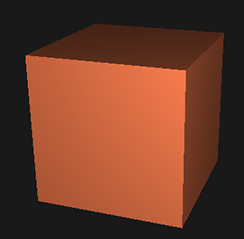
\includegraphics[width=0.2\linewidth]{img/1-4-1-flat.png}
    \caption{Пример плоской закраски }
    \label{fig:1-4-1-flat}
\end{figure}

\paragraph{Преимущества:}
\begin{itemize}
	\item[$-$] Очень высокая скорость обработки;
    \item[$-$] Простота реализации.
\end{itemize}
\paragraph{Недостатки:}
\begin{itemize}
	\item[$-$] Объекты выглядят угловатыми и нереалистичными;
    \item[$-$] Не учитываются плавные переходы света и тени между полигонами.
\end{itemize}

\subsection{Закраска по Гуро}

Метод Гуро (Gouraud Shading) использует интерполяцию интенсивности цвета между вершинами полигона. Интенсивности в вершинах вычисляются на основе нормалей и освещения, а затем плавно изменяются по поверхности.

\begin{figure}[H]
    \centering
    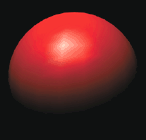
\includegraphics[width=0.2\linewidth]{img/1-4-2-gouraud.png}
    \caption{Пример закраски по Гуро}
    \label{fig:1-4-2-gouraud}
\end{figure}

\paragraph{Преимущества:}
\begin{itemize}
	\item[$-$] Плавные градиенты цвета между полигонами;
    \item[$-$] Улучшенное качество изображения по сравнению с плоской закраской.
\end{itemize}
\paragraph{Недостатки:}
\begin{itemize}
	\item[$-$] Возможна потеря детализации бликов, так как они могут не попадать на вершины;
    \item[$-$] Сложнее реализуется, чем простая закраска.
\end{itemize}

\subsection{Закраска по Фонгу}

Закраска по Фонгу (Phong Shading) интерполирует нормали между вершинами и вычисляет освещение для каждого пикселя, используя интерполированные нормали.

\begin{figure}[H]
    \centering
    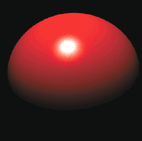
\includegraphics[width=0.2\linewidth]{img/1-4-3-phong.png}
    \caption{Пример закраски по Фонгу}
    \label{fig:1-4-3-phong}
\end{figure}

\paragraph{Преимущества:}
\begin{itemize}
	\item[$-$] Высокая реалистичность, особенно в отображении бликов;
    \item[$-$] Плавные и точные переходы света и тени.
\end{itemize}
\paragraph{Недостатки:}
\begin{itemize}
	\item[$-$] Более высокая вычислительная нагрузка;
    \item[$-$] Сложность реализации по сравнению с методом Гуро [4].
\end{itemize}

\subsection{Выбор алгоритма закраски}

В курсовой работе оптимальным выбором является закраска по Гуро, так как алгоритм обеспечивает достаточную реалистичность без значительного увеличения вычислительных затрат.

\section{Анализ моделей освещения}

Модель освещения определяет, как свет взаимодействует с поверхностями объектов, что существенно влияет на реализм сцены. Выделяют три основные модели освещения: модель Ламберта, модель
Фонга и модель Блинна$-$Фонга [5].

\subsection{Модель освещения Ламберта}

Модель Ламберта описывает идеальное диффузное отражение света от матовой поверхности. Интенсивность отраженного света зависит от косинуса угла между нормалью к поверхности и направлением на источник света.

\begin{figure}[h]
    \centering
    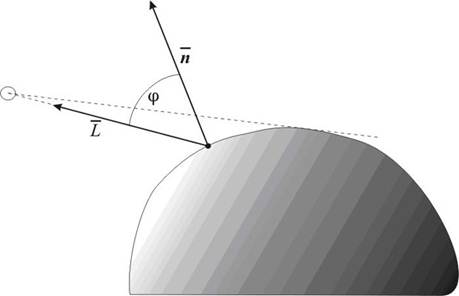
\includegraphics[width=0.3\linewidth]{img/1-5-1-lambert.jpg}
    \caption{Модель освещения Ламберта}
    \label{fig:1-5-1-lambert}
\end{figure}

\subsection{Модель освещения Фонга}

Модель Фонга расширяет модель Ламберта, добавляя зеркальную составляющую. Это позволяет отображать блики и более сложные эффекты освещения, делая объекты более реалистичными.

\begin{figure}[h]
    \centering
    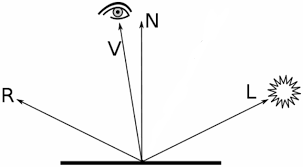
\includegraphics[width=0.3\linewidth]{img/1-5-2-phong.png}
    \caption{Модель освещения Фонга}
    \label{fig:1-5-2-phong}
\end{figure}

\subsection{Модель Блинна-Фонга}

В 1977 году Джеймсом Ф. Блинном была представлена модель освещения Блинна-Фонга, как дополнение к модели Фонга. Модель использует иной подход к расчету зеркальной компоненты. Вместо вектора отражения используется медианный вектор, который представляет из себя единичный вектор точно посередине между направлением обзора и направлением света. Чем ближе этот вектор к нормали поверхности, тем больше будет вклад зеркальной компоненты.

\begin{figure}[h]
    \centering
    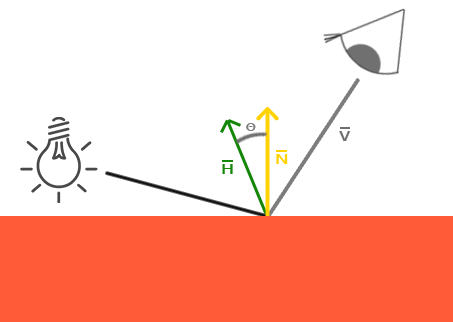
\includegraphics[width=0.3\linewidth]{img/1-5-3-blinnphong.png}
    \caption{Модель освещения Блинна-Фонга}
    \label{fig:1-5-2-phong}
\end{figure}

\subsection{Выбор модели освещения}

С учетом специфики курсовой работы, модель освещения Ламберта является наиболее подходящей.
Модель обеспечивает приемлемое качество освещения, легко реализуется и интегрируется с закраской по Гуро, а также менее требовательна к вычислительным ресурсам, что важно для поддержания производительности в реальном времени.

\vspace{15mm}

\textbf{ВЫВОД}

В данном разделе проведен анализ существующих алгоритмов построения изображений. Для решения задачи была выбрана поверхностная модель, алгоритм, использующий Z-буфер, закраска по Гуро и модель освещения Ламберта.